\chapter{控制器仿真以及实际飞行实验结果分析}
\label{chap:simulatin_expermient}
本章之中,按照第\ref{chap:controller_design}章中给出的控制器的数学模型,选定相应的初始条件进行双机的质点模型数学仿真:即不考虑无人机的姿态,只考虑无人机的位置,速度大小以及方向。之后,利用第\ref{chap:hardware}章中介绍的$ROS/Gazebo-PX4$仿真环境,在考虑无人机动力学的条件下进行双机编队仿真。
\section{基于MATLAB/Simulink的双机编队数学仿真}
本节数学仿真只验证编队控制器的控制性能以及控制逻辑的正确性,因而在仿真之前,做如下假设:
\begin{array}
\item 无人机自动驾驶仪内环仅为一个具有时间常数$\tau$一阶惯性环节。
\item 无人机的姿态动力学没有过渡过程,即姿态动力学方程由相应的稳态方程代替。
\end{array}
选取的初始条件均为在地面坐标系$NED$中定义:
领机初始位置$P_{0}^{l}=(0,100)$;
领机初始速度$V_{0}^{l}=(20,0)$;
从机的初始位置$P_{0}^{f}=(0,0)$;
从机的初始速度$V_{0}^{f}=(10,10)$;

\begin{figure}[H]
    \centering
    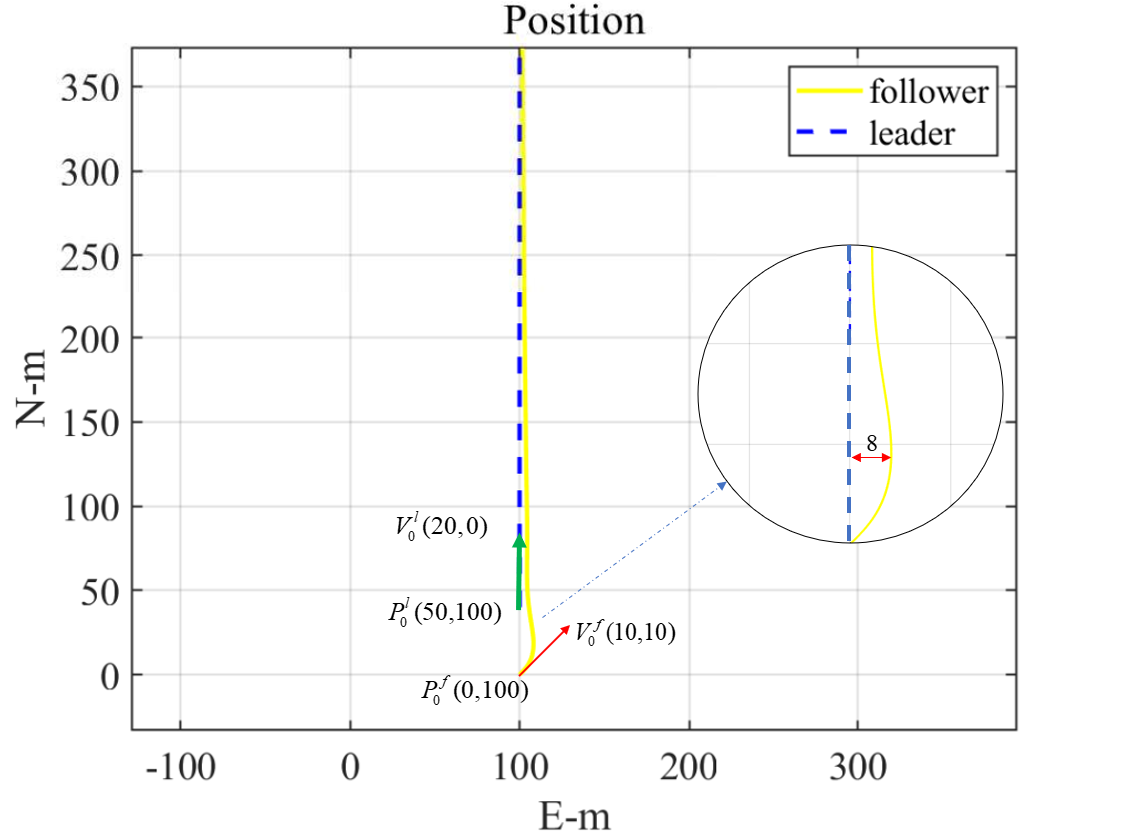
\includegraphics[width=0.85\textwidth]{figures/c5/c5-matlab-pos.png}
    \caption{双机编队位置关系}\label{fig:c5-matlab-pos}
\end{figure}
\section{基于ROS/Gazebo-PX4的双机编队动力学仿真}
